Als erstes wollen wir uns mit der Fourier-Analyse von Signalen besch"aftigen.
Hierbei ist das Ziel das Verhalten eines Signals im Frequenzbereich zu charakterisieren.
Wir wollen jedoch in unserer Analyse davon ausgehen, dass wir ein Signal $x[\cdot]$ vorliegen haben, dessen spektrale Eigenschaften \emph{zeitvariant} sind.
Hiermit ist \emph{nicht} gemeint, dass wir davon ausgehen, dass das Signal zeitvariant ist, denn das ist es nat"urlich.
Es geht darum, dass der Anteil der verschiedenen Frequenzen in einem Signal sich mit der Zeit "andert.
Nat"urlich ist hier eine der am einfachsten zug"anglichen Anwendungen die Analyse von Audiosignalen.

Beginnen wir mit einer intuitiven Betrachtung.
Zun"achst wollen wir einen m"oglichst gro"sen Bereich im Frequenzbereich abdecken -- zumindest den f"ur die jeweilige Anwendung relevanten.
Da sich beispielsweise im Audiobereich oft an der menschlichen H"orcharakteristik orientiert wird, die jenseits von \SI{20}{\kilo\hertz} nichts mehr leistet, sind Frequenzen jenseits dieser Grenze nicht mehr relevant.
Das hei"st, dass sinnvollerweise ein Audiosignal mit einer Sample-Rate von \SI{40}{\kilo\hertz} bereits absolut ausreichend aufgenommen wurde.
F"ur andere Anwendungen lassen sich oft "ahnliche Argumente finden, da die meisten physikalischen Systeme eine Tief- oder Bandpasscharakteristik \q{versteckt} haben, und man somit nur sehr selten mit Signalen mit immensen Bandbreiten konfrontiert ist.
Zusammenfassend muss also die Sample-Rate so angepasst werden, dass sie entsprechend unserer Anforderungen ausreicht.

Dar"uber hinaus ist uns aber auch gut daran getan, die Frequenzen, die in dem Signal vorkommen, sehr gut unterscheiden zu k"onnen.
Wir wollen also m"oglichst \emph{genau} wissen, welche einzelnen Frequenzen im Signal vorhanden sind. 
Das hei"st, dass wir f"ur eine tats"achlich im Signal vorhandene Frequenz $F$ aus unserer Analyse eine Frequenz erhalten wollen, die im Intervall $[F-\Delta_1,F-\Delta_1]$ f"ur m"oglichst kleines $\Delta_1 > 0$ liegt.
In diesem Sinne wollen wir also m"oglichst gro"se \emph{Aufl"osung}.
Wenn wir daran denken, dass $\Delta_1 = F_s/N$ gilt, so scheint es zu helfen, dass wir ein Signal m"oglichst lange \q{beobachten} m"ussen, also $N$ sehr gro"s w"ahlen m"ussen.

Doch es gibt noch einen weiteren Aufl"osungsbegriff, der vom ersten strikt zu unterscheiden ist.
Wir wollen au"serdem eine maximale Trennsch"arfe zwischen zwei unterschiedlichen Frequenzen, die gleichzeitig im Signal vorhanden sind, erreichen.
Wir wollen also in unserer Analyse zwei Frequenzen $F_1$ und $F_2$ mit $\Abs{F_1 - F_2} = \Delta_2$ immernoch unterscheiden k"onnen.
Wiederum ist hier das minimale $\Delta_2 > 0$ von Interesse, f"ur das diese Unterscheidbarkeit noch gilt, da dieses ein weiteres Aufl"osungslimit unseres Systems ist.
"Ahnlich wie bei $\Delta_1$ ist auch hier der Beobachtungszeitraum $N$, welchen wir als Grundlage f"ur unsere Analyse verwenden, von Bedeutung. 
Gr"o"ser Zeitr"aume erlauben eine bessere Aufl"osung \emph{zwischen} Frequenzen.

Au"serdem ist es noch oft interessant, dass man einen hohen Dynamikbereich abdecken kann.
Dies meint, dass man Frequenzanteile mit Frequenzen $F_1$ und $F_2$ und Amplituden $A_1$ und $A_2$ noch als zwei wahrnimmt, solange $\log(A_1/A_2) > \Delta_3$. 
Je gr"o"ser das maximale $\Delta_3$ ist, desto besser, da prominente Frequenzanteile nicht weitere weniger stark ausgepr"agte Anteile maskieren.

Schlussendlich haben wir es auch mit zeitvarianten Frequenzanteilen zu tun.
Das hei"st, dass sich zum Zeitpunkt $T_1$ die Zusammensetzung der Frequenzen von denen zum Zeitpunkt $T_2$ unterscheidet.
F"ur $\Abs{T_1 - T_2} > \Delta_4$ wollen wir also erkennen, dass $x(T_1)$ andere spektrale Charakteristik hat als $x(T_2)$ und die f"ur m"oglichst kleine $\Delta_4$.
Diese zeitliche Evolution des Spektrums ist nat"urlich von immenser Bedeutung, weil man m"oglichst genau wissen m"ochte, \emph{wann} sich Frequenzen im Signal ver"andern.
Ideal w"are es also, wenn wir eine Art \q{instantane} Frequenzanalyse durchf"uhren k"onnten, die trennscharf in einem infinitesimalen Intervall die jeweiligen Frequenzanteile aus dem Signal extrahiert.
Doch Schwingungen sind auf inh"arent \emph{ausgedehnte} Effekte.
Ein kleines $\Delta_4$ steht also in direktem Widerspruch zu den Anforderungen an unsere Analyse f"ur, gute (lies: kleine) $\Delta_1$ und $\Delta_2$, da wir dort gesehen haben, dass wir das Signal \emph{lange} beobachten m"ussen.
F"ur diesen Beobachtungszeitraum nehmen wir aber das Signal als \q{konstant} im Frequenzbereich -- also genau kontraproduktiv f"ur ein kleines $\Delta_4$.
\begin{listing}[ht]
    \noindent
    \begin{minipage}{0.51\textwidth}
        \strut\vspace*{-\baselineskip}\newline
        \inputminted[firstline=10, lastline=44]{python3}{code/stft_1.py}
    \end{minipage}%
    \begin{minipage}{0.48\textwidth}
        \strut\vspace*{-\baselineskip}\newline
        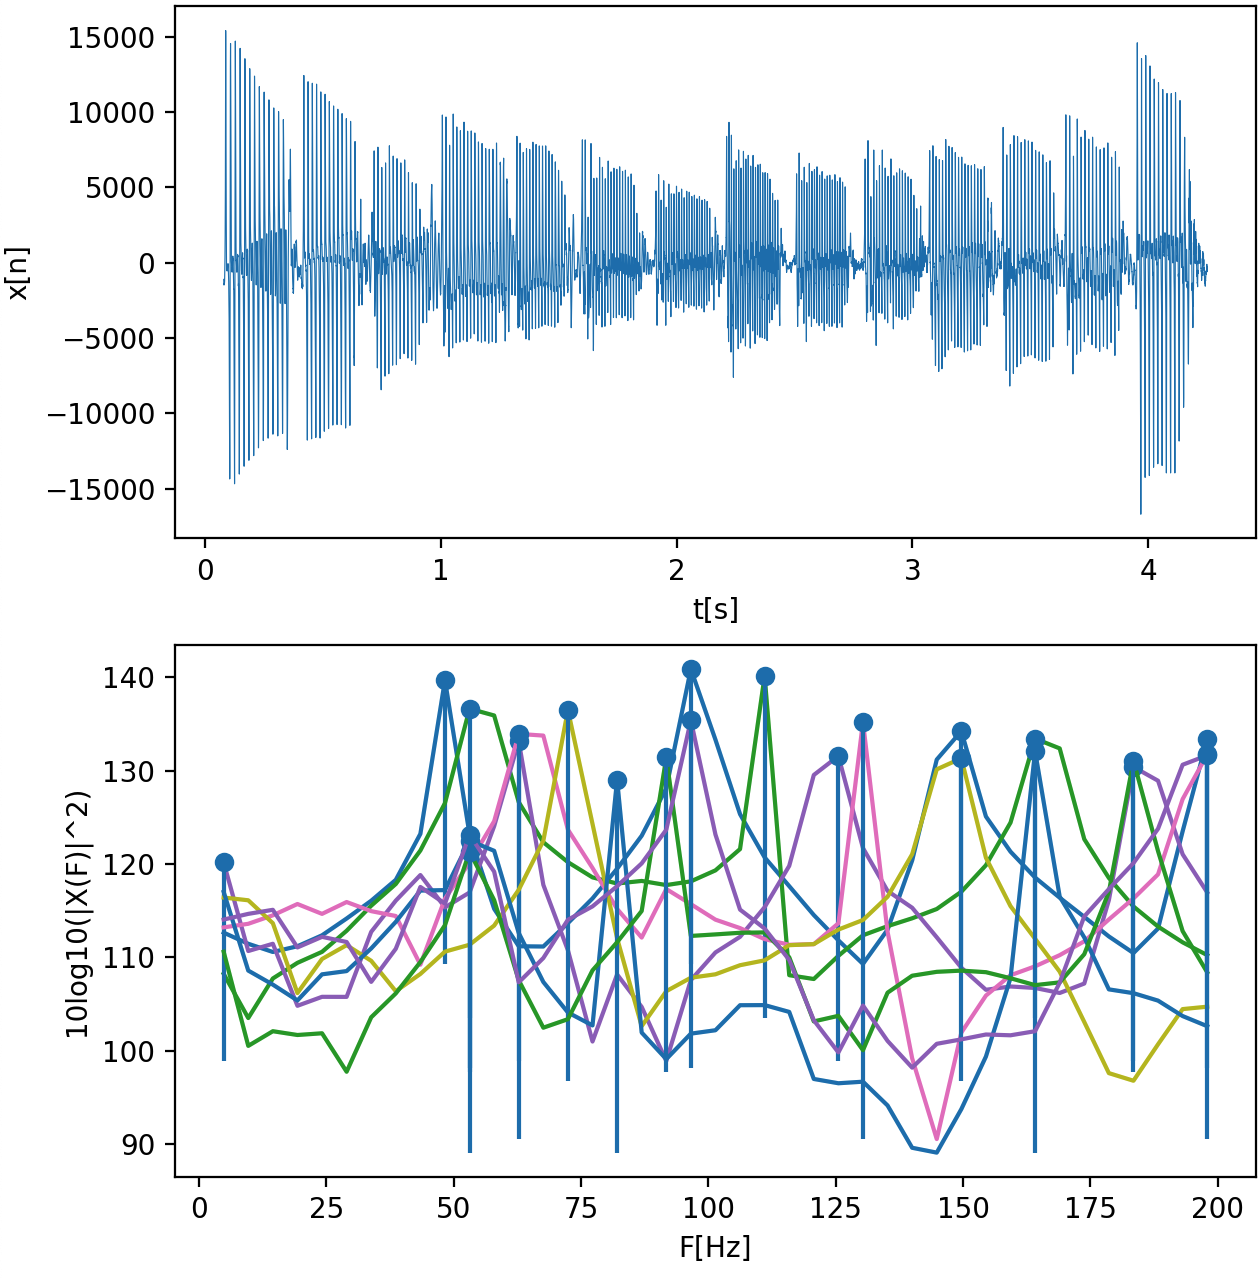
\includegraphics[width=\textwidth]{code/stft_1.png}

\begin{minted}{python}
[ 48.2811  96.5622 149.6715 197.9527]
[ 53.109  111.0466 164.1559]
[  4.8281  62.7654 125.5309 183.4683]
[ 62.7654 130.3590 197.9527]
[ 72.4217 149.6715]
[ 53.109   82.0779 164.1559]
[ 53.109   91.7341 183.4683]
[ 53.109   96.5622 197.95270418]
\end{minted}
    \end{minipage}
    \codecaption{dsv/code/stft_1.py}{Analyse einer \q{Bassline}, die eine G-Dur-Tonleiter spielt.}\label{py:stft_1}
\end{listing}

